\documentclass[twoside]{book}

% Packages required by doxygen
\usepackage{calc}
\usepackage{doxygen}
\usepackage{graphicx}
\usepackage[utf8]{inputenc}
\usepackage{makeidx}
\usepackage{multicol}
\usepackage{multirow}
\usepackage{textcomp}
\usepackage[table]{xcolor}

% Font selection
\usepackage[T1]{fontenc}
\usepackage{mathptmx}
\usepackage[scaled=.90]{helvet}
\usepackage{courier}
\usepackage{amssymb}
\usepackage{sectsty}
\renewcommand{\familydefault}{\sfdefault}
\allsectionsfont{%
  \fontseries{bc}\selectfont%
  \color{darkgray}%
}
\renewcommand{\DoxyLabelFont}{%
  \fontseries{bc}\selectfont%
  \color{darkgray}%
}

% Page & text layout
\usepackage{geometry}
\geometry{%
  a4paper,%
  top=2.5cm,%
  bottom=2.5cm,%
  left=2.5cm,%
  right=2.5cm%
}
\tolerance=750
\hfuzz=15pt
\hbadness=750
\setlength{\emergencystretch}{15pt}
\setlength{\parindent}{0cm}
\setlength{\parskip}{0.2cm}
\makeatletter
\renewcommand{\paragraph}{%
  \@startsection{paragraph}{4}{0ex}{-1.0ex}{1.0ex}{%
    \normalfont\normalsize\bfseries\SS@parafont%
  }%
}
\renewcommand{\subparagraph}{%
  \@startsection{subparagraph}{5}{0ex}{-1.0ex}{1.0ex}{%
    \normalfont\normalsize\bfseries\SS@subparafont%
  }%
}
\makeatother

% Headers & footers
\usepackage{fancyhdr}
\pagestyle{fancyplain}
\fancyhead[LE]{\fancyplain{}{\bfseries\thepage}}
\fancyhead[CE]{\fancyplain{}{}}
\fancyhead[RE]{\fancyplain{}{\bfseries\leftmark}}
\fancyhead[LO]{\fancyplain{}{\bfseries\rightmark}}
\fancyhead[CO]{\fancyplain{}{}}
\fancyhead[RO]{\fancyplain{}{\bfseries\thepage}}
\fancyfoot[LE]{\fancyplain{}{}}
\fancyfoot[CE]{\fancyplain{}{}}
\fancyfoot[RE]{\fancyplain{}{\bfseries\scriptsize Generated on Tue Jun 11 2013 22:49:49 for NostalgiaRoom by Doxygen }}
\fancyfoot[LO]{\fancyplain{}{\bfseries\scriptsize Generated on Tue Jun 11 2013 22:49:49 for NostalgiaRoom by Doxygen }}
\fancyfoot[CO]{\fancyplain{}{}}
\fancyfoot[RO]{\fancyplain{}{}}
\renewcommand{\footrulewidth}{0.4pt}
\renewcommand{\chaptermark}[1]{%
  \markboth{#1}{}%
}
\renewcommand{\sectionmark}[1]{%
  \markright{\thesection\ #1}%
}

% Indices & bibliography
\usepackage{natbib}
\usepackage[titles]{tocloft}
\setcounter{tocdepth}{3}
\setcounter{secnumdepth}{5}
\makeindex

% Hyperlinks (required, but should be loaded last)
\usepackage{ifpdf}
\ifpdf
  \usepackage[pdftex,pagebackref=true]{hyperref}
\else
  \usepackage[ps2pdf,pagebackref=true]{hyperref}
\fi
\hypersetup{%
  colorlinks=true,%
  linkcolor=blue,%
  citecolor=blue,%
  unicode%
}

% Custom commands
\newcommand{\clearemptydoublepage}{%
  \newpage{\pagestyle{empty}\cleardoublepage}%
}


%===== C O N T E N T S =====

\begin{document}

% Titlepage & ToC
\hypersetup{pageanchor=false}
\pagenumbering{roman}
\begin{titlepage}
\vspace*{7cm}
\begin{center}%
{\Large Nostalgia\-Room \\[1ex]\large 1.\-0 }\\
\vspace*{1cm}
{\large Generated by Doxygen 1.8.4}\\
\vspace*{0.5cm}
{\small Tue Jun 11 2013 22:49:49}\\
\end{center}
\end{titlepage}
\clearemptydoublepage
\tableofcontents
\clearemptydoublepage
\pagenumbering{arabic}
\hypersetup{pageanchor=true}

%--- Begin generated contents ---
\chapter{Hierarchical Index}
\section{Class Hierarchy}
This inheritance list is sorted roughly, but not completely, alphabetically\-:\begin{DoxyCompactList}
\item \contentsline{section}{Image\-Data}{\pageref{struct_image_data}}{}
\item of\-Base\-App\begin{DoxyCompactList}
\item \contentsline{section}{test\-App}{\pageref{classtest_app}}{}
\end{DoxyCompactList}
\end{DoxyCompactList}

\chapter{Class Index}
\section{Class List}
Here are the classes, structs, unions and interfaces with brief descriptions\-:\begin{DoxyCompactList}
\item\contentsline{section}{\hyperlink{struct_image_data}{Image\-Data} }{\pageref{struct_image_data}}{}
\item\contentsline{section}{\hyperlink{classtest_app}{test\-App} }{\pageref{classtest_app}}{}
\end{DoxyCompactList}

\chapter{File Index}
\section{File List}
Here is a list of all files with brief descriptions\-:\begin{DoxyCompactList}
\item\contentsline{section}{/\-Users/rahulbudhiraja/\-Work/of\-\_\-v0073\-\_\-osx\-\_\-release/apps/my\-Apps/\-Nostalgia\-\_\-\-Spiral/src/\hyperlink{main_8cpp}{main.\-cpp} }{\pageref{main_8cpp}}{}
\item\contentsline{section}{/\-Users/rahulbudhiraja/\-Work/of\-\_\-v0073\-\_\-osx\-\_\-release/apps/my\-Apps/\-Nostalgia\-\_\-\-Spiral/src/\hyperlink{test_app_8cpp}{test\-App.\-cpp} }{\pageref{test_app_8cpp}}{}
\item\contentsline{section}{/\-Users/rahulbudhiraja/\-Work/of\-\_\-v0073\-\_\-osx\-\_\-release/apps/my\-Apps/\-Nostalgia\-\_\-\-Spiral/src/\hyperlink{test_app_8h}{test\-App.\-h} }{\pageref{test_app_8h}}{}
\end{DoxyCompactList}

\chapter{Class Documentation}
\hypertarget{struct_image_data}{\section{Image\-Data Struct Reference}
\label{struct_image_data}\index{Image\-Data@{Image\-Data}}
}


{\ttfamily \#include $<$test\-App.\-h$>$}

\subsection*{Public Member Functions}
\begin{DoxyCompactItemize}
\item 
bool \hyperlink{struct_image_data_ab7ad50e15d1943523214dd8cc2cd7e01}{operator()} (const \hyperlink{struct_image_data}{Image\-Data} \&l, const \hyperlink{struct_image_data}{Image\-Data} \&m)
\end{DoxyCompactItemize}
\subsection*{Public Attributes}
\begin{DoxyCompactItemize}
\item 
float \hyperlink{struct_image_data_a7161728d2f1bd4240bd9359f6276dd3b}{image\-Score}
\item 
int \hyperlink{struct_image_data_a372655668350953b85fda1f07cd3ffe1}{albumnumber}
\item 
int \hyperlink{struct_image_data_a254eb9353be246c69591d51088683397}{image\-Number}
\item 
of\-Image \hyperlink{struct_image_data_acf1bde00dd79a0960269618d9b885f61}{theloadedimage}
\end{DoxyCompactItemize}


\subsection{Detailed Description}


Definition at line 34 of file test\-App.\-h.



\subsection{Member Function Documentation}
\hypertarget{struct_image_data_ab7ad50e15d1943523214dd8cc2cd7e01}{\index{Image\-Data@{Image\-Data}!operator()@{operator()}}
\index{operator()@{operator()}!ImageData@{Image\-Data}}
\subsubsection[{operator()}]{\setlength{\rightskip}{0pt plus 5cm}bool Image\-Data\-::operator() (
\begin{DoxyParamCaption}
\item[{const {\bf Image\-Data} \&}]{l, }
\item[{const {\bf Image\-Data} \&}]{m}
\end{DoxyParamCaption}
)\hspace{0.3cm}{\ttfamily [inline]}}}\label{struct_image_data_ab7ad50e15d1943523214dd8cc2cd7e01}


Definition at line 46 of file test\-App.\-h.



\subsection{Member Data Documentation}
\hypertarget{struct_image_data_a372655668350953b85fda1f07cd3ffe1}{\index{Image\-Data@{Image\-Data}!albumnumber@{albumnumber}}
\index{albumnumber@{albumnumber}!ImageData@{Image\-Data}}
\subsubsection[{albumnumber}]{\setlength{\rightskip}{0pt plus 5cm}int Image\-Data\-::albumnumber}}\label{struct_image_data_a372655668350953b85fda1f07cd3ffe1}


Definition at line 37 of file test\-App.\-h.

\hypertarget{struct_image_data_a254eb9353be246c69591d51088683397}{\index{Image\-Data@{Image\-Data}!image\-Number@{image\-Number}}
\index{image\-Number@{image\-Number}!ImageData@{Image\-Data}}
\subsubsection[{image\-Number}]{\setlength{\rightskip}{0pt plus 5cm}int Image\-Data\-::image\-Number}}\label{struct_image_data_a254eb9353be246c69591d51088683397}


Definition at line 38 of file test\-App.\-h.

\hypertarget{struct_image_data_a7161728d2f1bd4240bd9359f6276dd3b}{\index{Image\-Data@{Image\-Data}!image\-Score@{image\-Score}}
\index{image\-Score@{image\-Score}!ImageData@{Image\-Data}}
\subsubsection[{image\-Score}]{\setlength{\rightskip}{0pt plus 5cm}float Image\-Data\-::image\-Score}}\label{struct_image_data_a7161728d2f1bd4240bd9359f6276dd3b}


Definition at line 36 of file test\-App.\-h.

\hypertarget{struct_image_data_acf1bde00dd79a0960269618d9b885f61}{\index{Image\-Data@{Image\-Data}!theloadedimage@{theloadedimage}}
\index{theloadedimage@{theloadedimage}!ImageData@{Image\-Data}}
\subsubsection[{theloadedimage}]{\setlength{\rightskip}{0pt plus 5cm}of\-Image Image\-Data\-::theloadedimage}}\label{struct_image_data_acf1bde00dd79a0960269618d9b885f61}


Definition at line 41 of file test\-App.\-h.



The documentation for this struct was generated from the following file\-:\begin{DoxyCompactItemize}
\item 
\hyperlink{test_app_8h}{test\-App.\-h}\end{DoxyCompactItemize}

\hypertarget{classtest_app}{\section{test\-App Class Reference}
\label{classtest_app}\index{test\-App@{test\-App}}
}


{\ttfamily \#include $<$test\-App.\-h$>$}



Inheritance diagram for test\-App\-:\nopagebreak
\begin{figure}[H]
\begin{center}
\leavevmode
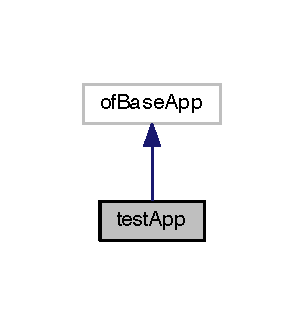
\includegraphics[width=146pt]{classtest_app__inherit__graph}
\end{center}
\end{figure}


Collaboration diagram for test\-App\-:\nopagebreak
\begin{figure}[H]
\begin{center}
\leavevmode
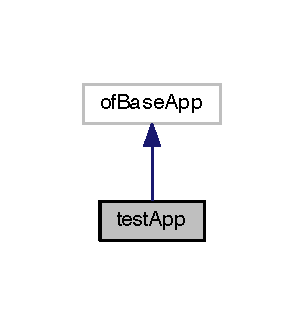
\includegraphics[width=146pt]{classtest_app__coll__graph}
\end{center}
\end{figure}
\subsection*{Public Member Functions}
\begin{DoxyCompactItemize}
\item 
void \hyperlink{group___openframeworks_defaults_gad431db15b6150b965cd52bcba8e16e11}{setup} ()
\item 
void \hyperlink{group___openframeworks_defaults_gafb39d201aec71a295b7609876bf7d0c6}{update} ()
\item 
void \hyperlink{group___openframeworks_defaults_gaf869cba67b1dab8481f8d0e216d59dcd}{draw} ()
\item 
void \hyperlink{group___openframeworks_defaults_ga904d147c7e532cb92656d5dd4895cd26}{key\-Pressed} (int key)
\item 
void \hyperlink{group___openframeworks_defaults_ga1116a10088e4932f6d482efe723cd45e}{key\-Released} (int key)
\item 
void \hyperlink{group___openframeworks_defaults_ga33541b19eff9f8285b2487bfc146d58b}{mouse\-Moved} (int x, int y)
\item 
void \hyperlink{group___openframeworks_defaults_ga075bcc2be16fd8f3eaa9162fb40a0a1f}{mouse\-Dragged} (int x, int y, int button)
\item 
void \hyperlink{group___openframeworks_defaults_ga3f200702ce91859cac2872a39302679d}{mouse\-Pressed} (int x, int y, int button)
\item 
void \hyperlink{group___openframeworks_defaults_gaa3680ffc782b1e5c451289817f20c9c6}{mouse\-Released} (int x, int y, int button)
\item 
void \hyperlink{group___openframeworks_defaults_ga428b7df9c64352d6e7cb234fc297e6c9}{window\-Resized} (int w, int h)
\item 
void \hyperlink{group___openframeworks_defaults_gaf15e9e9064fe5ccbe6c82cc401ae9e09}{drag\-Event} (of\-Drag\-Info drag\-Info)
\item 
void \hyperlink{classtest_app_a66dbc8c5c2d4e20febebe9fd42b8c851}{got\-Message} (of\-Message msg)
\item 
\hyperlink{classtest_app_a43cbf11b718251f1fff8fbbe4a24d517}{test\-App} (long long int id1)
\item 
of\-Vec3f \hyperlink{group___camera_animation_ga2a792bfdf269fd69951cbf97d4f574af}{adjustover\-Shot\-Camera\-Position} ()
\item 
of\-Vec3f \hyperlink{group___camera_animation_ga1facfe2200dae7ad147b8f9ab31f68c6}{animate} (int, int)
\item 
void \hyperlink{group___camera_animation_ga79467453f6ea0dd63961a810dca9ac6a}{start\-Animation} ()
\item 
of\-Vec3f \hyperlink{group___camera_animation_ga1a97063e992528dc79867e516d9365f0}{start\-Animation\-Camera\-Position} ()
\item 
void \hyperlink{group___wiggle_gaaa5c2175be1d5ca404c3c23a898d0cdd}{push\-Wiggle\-Positions} ()
\item 
of\-Vec3f \hyperlink{group___wiggle_gacd718eb54b9dc2b45e463414c24de6b9}{wiggle} ()
\item 
void \hyperlink{classtest_app_aa93380112b906e2aac2d8738309b2d17}{load\-Imagesand\-X\-M\-L\-Data} ()
\item 
void \hyperlink{classtest_app_a6dbcb5f1e47c842dfd1ab6b188097677}{draw\-Images} ()
\item 
void \hyperlink{classtest_app_aa30f4f1db2d186466f97e6ca15169712}{generate\-Circular\-Spiral} ()
\item 
void \hyperlink{group___drawing_stars_ga57e6d61c73ba0244b9d7a8c227aec244}{assign\-Star\-Positions} ()
\item 
void \hyperlink{group___drawing_stars_ga3ea688a73ca9eb760a3f0a07fde0ac10}{draw\-Stars} ()
\end{DoxyCompactItemize}
\subsection*{Public Attributes}
\begin{DoxyCompactItemize}
\item 
of\-Camera \hyperlink{group___camera_ga0278ee237cbbd881252d6273b131bb55}{camera}
\item 
of\-Vec3f \hyperlink{group___camera_gac01013264b9988207e7fd9e0a486ff2f}{camera\-Start\-Position}
\begin{DoxyCompactList}\small\item\em These variables will be useful if D\-E\-B\-U\-G\-M\-O\-D\-E is defined. \end{DoxyCompactList}\item 
of\-Vec3f \hyperlink{group___camera_gad3319d9cd3cb00e898f4f602b879efad}{camera\-End\-Position}
\item 
int \hyperlink{group___camera_ga4ca3a51642dedbf37f2b9f6ef96510c7}{cameraindex} =0
\begin{DoxyCompactList}\small\item\em The Cameraindex value,this make the camera go from one image/position to another. \end{DoxyCompactList}\item 
bool \hyperlink{group___camera_animation_ga2a5d49fd1f7f50f745f56095a1fa0099}{animation\-Mode}
\begin{DoxyCompactList}\small\item\em checks whether the camera is currently transitioning to another picture or if it is stationary a.\-k.\-a animation\-Mode \end{DoxyCompactList}\item 
float \hyperlink{group___camera_animation_gadd9ab1aa902948afbdf1c6db0dfde385}{tweenvalue}
\begin{DoxyCompactList}\small\item\em stores intermediate tweenvalues for all animations \end{DoxyCompactList}\item 
of\-Vec3f \hyperlink{group___camera_animation_gae9f60797c1c5d9f1ac06e1d6a5259957}{tweened\-Camera\-Position}
\begin{DoxyCompactList}\small\item\em Stores the temporary camera position while tweening(interpolating camera position while moving from 1 point in the spiral to another) \end{DoxyCompactList}\item 
int \hyperlink{group___camera_animation_ga21b16bdba744425519597fcb925df43a}{animation\-Counter}
\begin{DoxyCompactList}\small\item\em Animation Counter that is operative while the animation is occuring. \end{DoxyCompactList}\item 
bool \hyperlink{group___camera_animation_gab8a277e1055730fb5d6786ce0c4804b2}{isstarting\-Animation\-Active}
\begin{DoxyCompactList}\small\item\em If set,this variable will start the Animation of the spiral zooming out. \end{DoxyCompactList}\item 
int \hyperlink{group___camera_animation_ga577bf117cf10109de967ea0d3ca17f1f}{start\-Animation\-Counter}
\begin{DoxyCompactList}\small\item\em During the starting animation,the Start\-Animation\-Counter will change the tweenvalue which in turn sets the Camera\-Position. \end{DoxyCompactList}\item 
ofx\-Xml\-Settings \hyperlink{classtest_app_a85133f49103cfa002f39d882f7168236}{pictures\-\_\-\-X\-M\-L}
\begin{DoxyCompactList}\small\item\em To load the X\-M\-L File that is downloaded by the Nostalgia\-Room Website. \end{DoxyCompactList}\item 
long long int \hyperlink{classtest_app_a6ae76dc97fbeee00755f4a6cd6b87e19}{userid}
\begin{DoxyCompactList}\small\item\em The user's id that is passed at run-\/time.\-Only a long long int (max value 9223372036854775807) can support the range of the userids provided by Facebbok. \end{DoxyCompactList}\item 
vector$<$ of\-Vec3f $>$ \hyperlink{group___wiggle_ga5495d37f44bb3e3b00a04ad5910e0a6b}{wiggle\-Positions}
\item 
of\-Vec3f \hyperlink{group___wiggle_gaf81358868ae15faab1974ec074b1509f}{currentwiggle\-Position}
\begin{DoxyCompactList}\small\item\em Current Wiggle P\-Osition. \end{DoxyCompactList}\item 
int \hyperlink{group___wiggle_ga6b9af0b1ae4a2c0530eb6a8cf8340751}{currentwiggleindex}
\item 
float \hyperlink{group___wiggle_ga6073b33be7847d675ec089a1d514c506}{wiggle\-Animation\-Counter}
\item 
vector$<$ \hyperlink{struct_image_data}{Image\-Data} $>$ \hyperlink{classtest_app_aced9b8a8419c8465877c2c9cd43f8934}{combined\-Image\-Objects}
\begin{DoxyCompactList}\small\item\em The actual data structure that is used for storing the \hyperlink{struct_image_data}{Image\-Data} objects. \end{DoxyCompactList}\item 
vector$<$ of\-Vec3f $>$ \hyperlink{classtest_app_a68d0d30cea64a9d39a1b2deef16677ad}{Star\-Positions}
\begin{DoxyCompactList}\small\item\em Stores the positions of the stars. \end{DoxyCompactList}\item 
vector$<$ of\-Vec3f $>$ \hyperlink{classtest_app_af0dd2f3e3aabdb43bee49d74c156dc05}{Spiral\-Points}
\begin{DoxyCompactList}\small\item\em These are Spiralpoints generated using the Conical Helix function. \end{DoxyCompactList}\item 
vector$<$ of\-Image $>$ \hyperlink{classtest_app_ad4de5d6e6e8f3b8bb7424e62792deb1f}{Image\-Vector}
\begin{DoxyCompactList}\small\item\em Will store the loaded images from the directory in a Vector. \end{DoxyCompactList}\item 
int \hyperlink{classtest_app_a957cf7fdb3ea964a88ca1be13e4d68fc}{numberof\-Images}
\begin{DoxyCompactList}\small\item\em Number of images loaded in the Image\-Vector data structure. \end{DoxyCompactList}\item 
float \hyperlink{classtest_app_acb60fb8a89e9ec5d461630a20b11ceda}{timesince\-Last\-Transition}
\begin{DoxyCompactList}\small\item\em Time since Previous Transition/\-Animation. \end{DoxyCompactList}\item 
of\-Vec3f \hyperlink{classtest_app_a846feea7c2c4d4b1929bb72c546b3e19}{overshot\-Camera\-Starting\-Position}
\begin{DoxyCompactList}\small\item\em The whole starting Animation consists of a few Components.\-A video played at the start,The zooming out effect from the end of the spiral and an overshot animation that will take the Camera to the highest ranked image that will be shown first during the experience. The below data structures are for for the Overshot\-Camera\-Animation. \end{DoxyCompactList}\item 
bool \hyperlink{classtest_app_ad2fca6ce5e37462cd820afc48633324d}{startover\-Shot\-Camera\-Animation}
\begin{DoxyCompactList}\small\item\em When set,this will start the overshot camera animation. \end{DoxyCompactList}\item 
float \hyperlink{classtest_app_a808376783cdf510335cd1b37026e9bb3}{position1\-\_\-z}
\begin{DoxyCompactList}\small\item\em Intermediate values that are used while tweening/animation of the camera positions. \end{DoxyCompactList}\item 
float \hyperlink{classtest_app_a0720011cfaade6388109232ea4927c19}{position2\-\_\-z}
\item 
of\-Q\-T\-Kit\-Player \hyperlink{classtest_app_a9bfe7793fa0689a991ff64174745c38f}{starting\-Movie}
\begin{DoxyCompactList}\small\item\em Apparently,the of\-Q\-T\-Kit\-Player plays H\-D Video better than of\-Video\-Player. \end{DoxyCompactList}\item 
bool \hyperlink{classtest_app_aea3cb9f5f0061a42a4953d6b6c949036}{starting\-Movie\-Finished}
\begin{DoxyCompactList}\small\item\em Variable determines if the starting\-Movie has finished playing or not (initially set to false ) \end{DoxyCompactList}\item 
of\-Sound\-Player \hyperlink{classtest_app_af696fd13ee9ecb38ac0ba0b72543ce06}{Bluementhal\-Mp3}
\begin{DoxyCompactList}\small\item\em This class plays the Bluementhal song by Ulrich Schnauss in the background while the user watches his/her pictures.\-It is. \end{DoxyCompactList}\item 
float \hyperlink{group___wii_mote_ga020730abb55e6ae6d0a28edee19050e0}{roll}
\begin{DoxyCompactList}\small\item\em Roll,Yaw and Pitch as sent by O\-S\-Culator. \end{DoxyCompactList}\item 
float \hyperlink{group___wii_mote_ga865985f78dd5def3ed20c87b9fc772b6}{yaw}
\item 
float \hyperlink{group___wii_mote_gaabbebeb113838374f659e86a0355b260}{pitch}
\item 
float \hyperlink{group___wii_mote_ga8e560e923c82d421857538e4a5927542}{accel}
\item 
float \hyperlink{group___wii_mote_ga7a77e8633c3a94e3e409a33a5cd9ae3f}{wii\-X}
\item 
float \hyperlink{group___wii_mote_ga5ae41896388ae16ee530beca5333e02a}{wii\-Y}
\item 
float \hyperlink{group___wii_mote_gad1738ff98d225f80b853a9ddc9f5a116}{accel\-\_\-x}
\begin{DoxyCompactList}\small\item\em Acceleration in x,y and z. \end{DoxyCompactList}\item 
float \hyperlink{group___wii_mote_ga204bcb2412a70a65ebea6008ee8c4eb0}{accel\-\_\-y}
\item 
float \hyperlink{group___wii_mote_ga61dbdd5c0b868568dde40a52f6e56054}{accel\-\_\-z}
\item 
float \hyperlink{group___wii_mote_ga98e05c3206ff95fccfebfc9df5317598}{angular\-\_\-velocity}
\begin{DoxyCompactList}\small\item\em Angular Velocity as received from O\-S\-Culator ,this variable is helpful to predict if the swing is going forwards or backward .A +ve value means the swing is going front and a -\/ve value indicates the person is swinging backwards. \end{DoxyCompactList}\item 
ofx\-Osc\-Receiver \hyperlink{group___wii_mote_ga034c44ff60fa1e5f021e90d5410ba657}{receiver}
\begin{DoxyCompactList}\small\item\em O\-S\-C\-Receiver class that interfaces with the O\-S\-Culator and receives values from the wii-\/mote. \end{DoxyCompactList}\item 
string \hyperlink{group___wii_mote_ga0124035d0454fb6bd9152f8a87c40677}{Message}
\begin{DoxyCompactList}\small\item\em The message received from O\-S\-Culator containing details of the wiimote values like angular velocity and acceleration. \end{DoxyCompactList}\item 
int \hyperlink{group___wii_mote_ga9ed611377cd46f5148a3a3d538e96484}{window\-Width}
\item 
int \hyperlink{group___wii_mote_ga4e8884eeef5b2657b62278969d4e3dcf}{window\-Height}
\item 
float \hyperlink{group___wii_mote_ga8a2b9b9cf76097e20f148b616297029b}{prev\-Ang\-Vel} =0
\item 
float \hyperlink{classtest_app_ac559756a01e0b98378bc29dfba9fac79}{min\-Angular\-Velocity}
\begin{DoxyCompactList}\small\item\em These are the wii-\/mote variables that are used to adjust the timegap between two images. \end{DoxyCompactList}\item 
float \hyperlink{classtest_app_ab9565e8e6dc748ef68e6845f5f94cae9}{max\-Angular\-Velocity}
\item 
float \hyperlink{classtest_app_ab007edbc20b09d607f8010e2dbafdb97}{min\-Accel}
\item 
float \hyperlink{classtest_app_a34e834a5e4d359700147a74eece8eed1}{max\-Accel}
\item 
of\-True\-Type\-Font \hyperlink{classtest_app_ab336e228840f001d15f9b1eb3a30972f}{fonttodisplay\-Wiimote\-Values}
\begin{DoxyCompactList}\small\item\em Font to display the wiimote values on screen for debugging. \end{DoxyCompactList}\item 
string \hyperlink{classtest_app_a8ce5505df4526abed238956b65956edd}{State}
\begin{DoxyCompactList}\small\item\em Swing's current state i.\-e. \end{DoxyCompactList}\item 
float \hyperlink{classtest_app_a944f2713019239a4b49241a5cc9a00c9}{time\-Gap}
\begin{DoxyCompactList}\small\item\em Time that an image will be shown on the screen,this is controlled by the wii-\/motes acceleration. \end{DoxyCompactList}\item 
bool \hyperlink{classtest_app_a42478a80a90ce9f663c04bcdaea5c5bd}{isturn\-Completed}
\begin{DoxyCompactList}\small\item\em This variable is used to check if a half-\/swing is completed ,that is from back to front or from front to back. \end{DoxyCompactList}\item 
bool \hyperlink{classtest_app_a918c09b5a4389a8402cfacb25d390226}{fade\-Audio}
\begin{DoxyCompactList}\small\item\em If set,this variable will cause the current\-Volume variable to fade. \end{DoxyCompactList}\item 
float \hyperlink{classtest_app_a51c20c5432d9f6b06f719526d9a34ee6}{current\-Volume}
\begin{DoxyCompactList}\small\item\em The current volume variable is generally set to 1 ,but if fade\-Audio is enabled,it will reduce the audio by -\/0.\-001 every frame,this is used in the end along with the Corresponding video to reduce the volume of the music. \end{DoxyCompactList}\item 
bool \hyperlink{classtest_app_a8a65a6d1a473417cec1c2ac2e6116aae}{start\-Installation}
\begin{DoxyCompactList}\small\item\em This variable is used to start the installation if the user is swinging on the wii-\/mote or if the enter key is pressed. \end{DoxyCompactList}\item 
of\-True\-Type\-Font \hyperlink{classtest_app_af5b1af55af2256ef3751de075fc7a9cc}{preview\-Text}
\begin{DoxyCompactList}\small\item\em preview\-Text is used for loading the font Asyouwish.\-ttf \end{DoxyCompactList}\item 
string \hyperlink{classtest_app_ad9a4beab6f2e0f13d32b00b502e89bdc}{temp\-Text}
\begin{DoxyCompactList}\small\item\em This string will display \char`\"{}\-Start Swinging !\char`\"{} at the start. \end{DoxyCompactList}\item 
bool \hyperlink{classtest_app_acf09303bc452d2a38098f6bf94655408}{ending}
\begin{DoxyCompactList}\small\item\em If true,the ending variable will trigger the backward playing of the starting video and provides a nice smooth ending. \end{DoxyCompactList}\item 
vector$<$ \hyperlink{struct_image_data}{Image\-Data} $>$ \hyperlink{classtest_app_af65c8dc2f4620bfe7fdf6a39043cb48d}{tagged\-Image\-Objects}
\begin{DoxyCompactList}\small\item\em Unused. \end{DoxyCompactList}\end{DoxyCompactItemize}


\subsection{Detailed Description}


Definition at line 45 of file test\-App.\-h.



\subsection{Constructor \& Destructor Documentation}
\hypertarget{classtest_app_a43cbf11b718251f1fff8fbbe4a24d517}{\index{test\-App@{test\-App}!test\-App@{test\-App}}
\index{test\-App@{test\-App}!testApp@{test\-App}}
\subsubsection[{test\-App}]{\setlength{\rightskip}{0pt plus 5cm}test\-App\-::test\-App (
\begin{DoxyParamCaption}
\item[{long long int}]{id1}
\end{DoxyParamCaption}
)}}\label{classtest_app_a43cbf11b718251f1fff8fbbe4a24d517}


Definition at line 602 of file test\-App.\-cpp.



\subsection{Member Function Documentation}
\hypertarget{classtest_app_a6dbcb5f1e47c842dfd1ab6b188097677}{\index{test\-App@{test\-App}!draw\-Images@{draw\-Images}}
\index{draw\-Images@{draw\-Images}!testApp@{test\-App}}
\subsubsection[{draw\-Images}]{\setlength{\rightskip}{0pt plus 5cm}void test\-App\-::draw\-Images (
\begin{DoxyParamCaption}
{}
\end{DoxyParamCaption}
)}}\label{classtest_app_a6dbcb5f1e47c842dfd1ab6b188097677}
This function will draw the images.\-Used in draw 

Definition at line 505 of file test\-App.\-cpp.

\hypertarget{classtest_app_aa30f4f1db2d186466f97e6ca15169712}{\index{test\-App@{test\-App}!generate\-Circular\-Spiral@{generate\-Circular\-Spiral}}
\index{generate\-Circular\-Spiral@{generate\-Circular\-Spiral}!testApp@{test\-App}}
\subsubsection[{generate\-Circular\-Spiral}]{\setlength{\rightskip}{0pt plus 5cm}void test\-App\-::generate\-Circular\-Spiral (
\begin{DoxyParamCaption}
{}
\end{DoxyParamCaption}
)}}\label{classtest_app_aa30f4f1db2d186466f97e6ca15169712}
Function that will generate the points on the Spiral 

Definition at line 470 of file test\-App.\-cpp.

\hypertarget{classtest_app_a66dbc8c5c2d4e20febebe9fd42b8c851}{\index{test\-App@{test\-App}!got\-Message@{got\-Message}}
\index{got\-Message@{got\-Message}!testApp@{test\-App}}
\subsubsection[{got\-Message}]{\setlength{\rightskip}{0pt plus 5cm}void test\-App\-::got\-Message (
\begin{DoxyParamCaption}
\item[{of\-Message}]{msg}
\end{DoxyParamCaption}
)}}\label{classtest_app_a66dbc8c5c2d4e20febebe9fd42b8c851}


Definition at line 461 of file test\-App.\-cpp.

\hypertarget{classtest_app_aa93380112b906e2aac2d8738309b2d17}{\index{test\-App@{test\-App}!load\-Imagesand\-X\-M\-L\-Data@{load\-Imagesand\-X\-M\-L\-Data}}
\index{load\-Imagesand\-X\-M\-L\-Data@{load\-Imagesand\-X\-M\-L\-Data}!testApp@{test\-App}}
\subsubsection[{load\-Imagesand\-X\-M\-L\-Data}]{\setlength{\rightskip}{0pt plus 5cm}void test\-App\-::load\-Imagesand\-X\-M\-L\-Data (
\begin{DoxyParamCaption}
{}
\end{DoxyParamCaption}
)}}\label{classtest_app_aa93380112b906e2aac2d8738309b2d17}
Load the Images and X\-M\-L Data.\-This function will load the images from the directory and then parse the xml to get the score and album number.\-Once that is done ,we combine the untagged and tagged images to get a combined Data Structure 

Definition at line 681 of file test\-App.\-cpp.



\subsection{Member Data Documentation}
\hypertarget{classtest_app_af696fd13ee9ecb38ac0ba0b72543ce06}{\index{test\-App@{test\-App}!Bluementhal\-Mp3@{Bluementhal\-Mp3}}
\index{Bluementhal\-Mp3@{Bluementhal\-Mp3}!testApp@{test\-App}}
\subsubsection[{Bluementhal\-Mp3}]{\setlength{\rightskip}{0pt plus 5cm}of\-Sound\-Player test\-App\-::\-Bluementhal\-Mp3}}\label{classtest_app_af696fd13ee9ecb38ac0ba0b72543ce06}


This class plays the Bluementhal song by Ulrich Schnauss in the background while the user watches his/her pictures.\-It is. 



Definition at line 184 of file test\-App.\-h.

\hypertarget{classtest_app_aced9b8a8419c8465877c2c9cd43f8934}{\index{test\-App@{test\-App}!combined\-Image\-Objects@{combined\-Image\-Objects}}
\index{combined\-Image\-Objects@{combined\-Image\-Objects}!testApp@{test\-App}}
\subsubsection[{combined\-Image\-Objects}]{\setlength{\rightskip}{0pt plus 5cm}vector$<${\bf Image\-Data}$>$ test\-App\-::combined\-Image\-Objects}}\label{classtest_app_aced9b8a8419c8465877c2c9cd43f8934}


The actual data structure that is used for storing the \hyperlink{struct_image_data}{Image\-Data} objects. 



Definition at line 144 of file test\-App.\-h.

\hypertarget{classtest_app_a51c20c5432d9f6b06f719526d9a34ee6}{\index{test\-App@{test\-App}!current\-Volume@{current\-Volume}}
\index{current\-Volume@{current\-Volume}!testApp@{test\-App}}
\subsubsection[{current\-Volume}]{\setlength{\rightskip}{0pt plus 5cm}float test\-App\-::current\-Volume}}\label{classtest_app_a51c20c5432d9f6b06f719526d9a34ee6}


The current volume variable is generally set to 1 ,but if fade\-Audio is enabled,it will reduce the audio by -\/0.\-001 every frame,this is used in the end along with the Corresponding video to reduce the volume of the music. 



Definition at line 243 of file test\-App.\-h.

\hypertarget{classtest_app_acf09303bc452d2a38098f6bf94655408}{\index{test\-App@{test\-App}!ending@{ending}}
\index{ending@{ending}!testApp@{test\-App}}
\subsubsection[{ending}]{\setlength{\rightskip}{0pt plus 5cm}bool test\-App\-::ending}}\label{classtest_app_acf09303bc452d2a38098f6bf94655408}


If true,the ending variable will trigger the backward playing of the starting video and provides a nice smooth ending. 



Definition at line 259 of file test\-App.\-h.

\hypertarget{classtest_app_a918c09b5a4389a8402cfacb25d390226}{\index{test\-App@{test\-App}!fade\-Audio@{fade\-Audio}}
\index{fade\-Audio@{fade\-Audio}!testApp@{test\-App}}
\subsubsection[{fade\-Audio}]{\setlength{\rightskip}{0pt plus 5cm}bool test\-App\-::fade\-Audio}}\label{classtest_app_a918c09b5a4389a8402cfacb25d390226}


If set,this variable will cause the current\-Volume variable to fade. 



Definition at line 240 of file test\-App.\-h.

\hypertarget{classtest_app_ab336e228840f001d15f9b1eb3a30972f}{\index{test\-App@{test\-App}!fonttodisplay\-Wiimote\-Values@{fonttodisplay\-Wiimote\-Values}}
\index{fonttodisplay\-Wiimote\-Values@{fonttodisplay\-Wiimote\-Values}!testApp@{test\-App}}
\subsubsection[{fonttodisplay\-Wiimote\-Values}]{\setlength{\rightskip}{0pt plus 5cm}of\-True\-Type\-Font test\-App\-::fonttodisplay\-Wiimote\-Values}}\label{classtest_app_ab336e228840f001d15f9b1eb3a30972f}


Font to display the wiimote values on screen for debugging. 



Definition at line 226 of file test\-App.\-h.

\hypertarget{classtest_app_ad4de5d6e6e8f3b8bb7424e62792deb1f}{\index{test\-App@{test\-App}!Image\-Vector@{Image\-Vector}}
\index{Image\-Vector@{Image\-Vector}!testApp@{test\-App}}
\subsubsection[{Image\-Vector}]{\setlength{\rightskip}{0pt plus 5cm}vector$<$of\-Image$>$ test\-App\-::\-Image\-Vector}}\label{classtest_app_ad4de5d6e6e8f3b8bb7424e62792deb1f}


Will store the loaded images from the directory in a Vector. 



Definition at line 156 of file test\-App.\-h.

\hypertarget{classtest_app_a42478a80a90ce9f663c04bcdaea5c5bd}{\index{test\-App@{test\-App}!isturn\-Completed@{isturn\-Completed}}
\index{isturn\-Completed@{isturn\-Completed}!testApp@{test\-App}}
\subsubsection[{isturn\-Completed}]{\setlength{\rightskip}{0pt plus 5cm}bool test\-App\-::isturn\-Completed}}\label{classtest_app_a42478a80a90ce9f663c04bcdaea5c5bd}


This variable is used to check if a half-\/swing is completed ,that is from back to front or from front to back. 



Definition at line 237 of file test\-App.\-h.

\hypertarget{classtest_app_a34e834a5e4d359700147a74eece8eed1}{\index{test\-App@{test\-App}!max\-Accel@{max\-Accel}}
\index{max\-Accel@{max\-Accel}!testApp@{test\-App}}
\subsubsection[{max\-Accel}]{\setlength{\rightskip}{0pt plus 5cm}float test\-App\-::max\-Accel}}\label{classtest_app_a34e834a5e4d359700147a74eece8eed1}


Definition at line 222 of file test\-App.\-h.

\hypertarget{classtest_app_ab9565e8e6dc748ef68e6845f5f94cae9}{\index{test\-App@{test\-App}!max\-Angular\-Velocity@{max\-Angular\-Velocity}}
\index{max\-Angular\-Velocity@{max\-Angular\-Velocity}!testApp@{test\-App}}
\subsubsection[{max\-Angular\-Velocity}]{\setlength{\rightskip}{0pt plus 5cm}float test\-App\-::max\-Angular\-Velocity}}\label{classtest_app_ab9565e8e6dc748ef68e6845f5f94cae9}


Definition at line 221 of file test\-App.\-h.

\hypertarget{classtest_app_ab007edbc20b09d607f8010e2dbafdb97}{\index{test\-App@{test\-App}!min\-Accel@{min\-Accel}}
\index{min\-Accel@{min\-Accel}!testApp@{test\-App}}
\subsubsection[{min\-Accel}]{\setlength{\rightskip}{0pt plus 5cm}float test\-App\-::min\-Accel}}\label{classtest_app_ab007edbc20b09d607f8010e2dbafdb97}


Definition at line 222 of file test\-App.\-h.

\hypertarget{classtest_app_ac559756a01e0b98378bc29dfba9fac79}{\index{test\-App@{test\-App}!min\-Angular\-Velocity@{min\-Angular\-Velocity}}
\index{min\-Angular\-Velocity@{min\-Angular\-Velocity}!testApp@{test\-App}}
\subsubsection[{min\-Angular\-Velocity}]{\setlength{\rightskip}{0pt plus 5cm}float test\-App\-::min\-Angular\-Velocity}}\label{classtest_app_ac559756a01e0b98378bc29dfba9fac79}


These are the wii-\/mote variables that are used to adjust the timegap between two images. 



Definition at line 221 of file test\-App.\-h.

\hypertarget{classtest_app_a957cf7fdb3ea964a88ca1be13e4d68fc}{\index{test\-App@{test\-App}!numberof\-Images@{numberof\-Images}}
\index{numberof\-Images@{numberof\-Images}!testApp@{test\-App}}
\subsubsection[{numberof\-Images}]{\setlength{\rightskip}{0pt plus 5cm}int test\-App\-::numberof\-Images}}\label{classtest_app_a957cf7fdb3ea964a88ca1be13e4d68fc}


Number of images loaded in the Image\-Vector data structure. 



Definition at line 159 of file test\-App.\-h.

\hypertarget{classtest_app_a846feea7c2c4d4b1929bb72c546b3e19}{\index{test\-App@{test\-App}!overshot\-Camera\-Starting\-Position@{overshot\-Camera\-Starting\-Position}}
\index{overshot\-Camera\-Starting\-Position@{overshot\-Camera\-Starting\-Position}!testApp@{test\-App}}
\subsubsection[{overshot\-Camera\-Starting\-Position}]{\setlength{\rightskip}{0pt plus 5cm}of\-Vec3f test\-App\-::overshot\-Camera\-Starting\-Position}}\label{classtest_app_a846feea7c2c4d4b1929bb72c546b3e19}


The whole starting Animation consists of a few Components.\-A video played at the start,The zooming out effect from the end of the spiral and an overshot animation that will take the Camera to the highest ranked image that will be shown first during the experience. The below data structures are for for the Overshot\-Camera\-Animation. 

This vector will store the overshot\-Camera\-Position and changes the camera\-Position during the start while tweening 

Definition at line 167 of file test\-App.\-h.

\hypertarget{classtest_app_a85133f49103cfa002f39d882f7168236}{\index{test\-App@{test\-App}!pictures\-\_\-\-X\-M\-L@{pictures\-\_\-\-X\-M\-L}}
\index{pictures\-\_\-\-X\-M\-L@{pictures\-\_\-\-X\-M\-L}!testApp@{test\-App}}
\subsubsection[{pictures\-\_\-\-X\-M\-L}]{\setlength{\rightskip}{0pt plus 5cm}ofx\-Xml\-Settings test\-App\-::pictures\-\_\-\-X\-M\-L}}\label{classtest_app_a85133f49103cfa002f39d882f7168236}


To load the X\-M\-L File that is downloaded by the Nostalgia\-Room Website. 



Definition at line 120 of file test\-App.\-h.

\hypertarget{classtest_app_a808376783cdf510335cd1b37026e9bb3}{\index{test\-App@{test\-App}!position1\-\_\-z@{position1\-\_\-z}}
\index{position1\-\_\-z@{position1\-\_\-z}!testApp@{test\-App}}
\subsubsection[{position1\-\_\-z}]{\setlength{\rightskip}{0pt plus 5cm}float test\-App\-::position1\-\_\-z}}\label{classtest_app_a808376783cdf510335cd1b37026e9bb3}


Intermediate values that are used while tweening/animation of the camera positions. 



Definition at line 175 of file test\-App.\-h.

\hypertarget{classtest_app_a0720011cfaade6388109232ea4927c19}{\index{test\-App@{test\-App}!position2\-\_\-z@{position2\-\_\-z}}
\index{position2\-\_\-z@{position2\-\_\-z}!testApp@{test\-App}}
\subsubsection[{position2\-\_\-z}]{\setlength{\rightskip}{0pt plus 5cm}float test\-App\-::position2\-\_\-z}}\label{classtest_app_a0720011cfaade6388109232ea4927c19}


Definition at line 175 of file test\-App.\-h.

\hypertarget{classtest_app_af5b1af55af2256ef3751de075fc7a9cc}{\index{test\-App@{test\-App}!preview\-Text@{preview\-Text}}
\index{preview\-Text@{preview\-Text}!testApp@{test\-App}}
\subsubsection[{preview\-Text}]{\setlength{\rightskip}{0pt plus 5cm}of\-True\-Type\-Font test\-App\-::preview\-Text}}\label{classtest_app_af5b1af55af2256ef3751de075fc7a9cc}


preview\-Text is used for loading the font Asyouwish.\-ttf 



Definition at line 253 of file test\-App.\-h.

\hypertarget{classtest_app_af0dd2f3e3aabdb43bee49d74c156dc05}{\index{test\-App@{test\-App}!Spiral\-Points@{Spiral\-Points}}
\index{Spiral\-Points@{Spiral\-Points}!testApp@{test\-App}}
\subsubsection[{Spiral\-Points}]{\setlength{\rightskip}{0pt plus 5cm}vector$<$of\-Vec3f$>$ test\-App\-::\-Spiral\-Points}}\label{classtest_app_af0dd2f3e3aabdb43bee49d74c156dc05}


These are Spiralpoints generated using the Conical Helix function. 



Definition at line 152 of file test\-App.\-h.

\hypertarget{classtest_app_a68d0d30cea64a9d39a1b2deef16677ad}{\index{test\-App@{test\-App}!Star\-Positions@{Star\-Positions}}
\index{Star\-Positions@{Star\-Positions}!testApp@{test\-App}}
\subsubsection[{Star\-Positions}]{\setlength{\rightskip}{0pt plus 5cm}vector$<$of\-Vec3f$>$ test\-App\-::\-Star\-Positions}}\label{classtest_app_a68d0d30cea64a9d39a1b2deef16677ad}


Stores the positions of the stars. 



Definition at line 147 of file test\-App.\-h.

\hypertarget{classtest_app_a9bfe7793fa0689a991ff64174745c38f}{\index{test\-App@{test\-App}!starting\-Movie@{starting\-Movie}}
\index{starting\-Movie@{starting\-Movie}!testApp@{test\-App}}
\subsubsection[{starting\-Movie}]{\setlength{\rightskip}{0pt plus 5cm}of\-Q\-T\-Kit\-Player test\-App\-::starting\-Movie}}\label{classtest_app_a9bfe7793fa0689a991ff64174745c38f}


Apparently,the of\-Q\-T\-Kit\-Player plays H\-D Video better than of\-Video\-Player. 



Definition at line 178 of file test\-App.\-h.

\hypertarget{classtest_app_aea3cb9f5f0061a42a4953d6b6c949036}{\index{test\-App@{test\-App}!starting\-Movie\-Finished@{starting\-Movie\-Finished}}
\index{starting\-Movie\-Finished@{starting\-Movie\-Finished}!testApp@{test\-App}}
\subsubsection[{starting\-Movie\-Finished}]{\setlength{\rightskip}{0pt plus 5cm}bool test\-App\-::starting\-Movie\-Finished}}\label{classtest_app_aea3cb9f5f0061a42a4953d6b6c949036}


Variable determines if the starting\-Movie has finished playing or not (initially set to false ) 



Definition at line 181 of file test\-App.\-h.

\hypertarget{classtest_app_a8a65a6d1a473417cec1c2ac2e6116aae}{\index{test\-App@{test\-App}!start\-Installation@{start\-Installation}}
\index{start\-Installation@{start\-Installation}!testApp@{test\-App}}
\subsubsection[{start\-Installation}]{\setlength{\rightskip}{0pt plus 5cm}bool test\-App\-::start\-Installation}}\label{classtest_app_a8a65a6d1a473417cec1c2ac2e6116aae}


This variable is used to start the installation if the user is swinging on the wii-\/mote or if the enter key is pressed. 



Definition at line 246 of file test\-App.\-h.

\hypertarget{classtest_app_ad2fca6ce5e37462cd820afc48633324d}{\index{test\-App@{test\-App}!startover\-Shot\-Camera\-Animation@{startover\-Shot\-Camera\-Animation}}
\index{startover\-Shot\-Camera\-Animation@{startover\-Shot\-Camera\-Animation}!testApp@{test\-App}}
\subsubsection[{startover\-Shot\-Camera\-Animation}]{\setlength{\rightskip}{0pt plus 5cm}bool test\-App\-::startover\-Shot\-Camera\-Animation}}\label{classtest_app_ad2fca6ce5e37462cd820afc48633324d}


When set,this will start the overshot camera animation. 



Definition at line 172 of file test\-App.\-h.

\hypertarget{classtest_app_a8ce5505df4526abed238956b65956edd}{\index{test\-App@{test\-App}!State@{State}}
\index{State@{State}!testApp@{test\-App}}
\subsubsection[{State}]{\setlength{\rightskip}{0pt plus 5cm}string test\-App\-::\-State}}\label{classtest_app_a8ce5505df4526abed238956b65956edd}


Swing's current state i.\-e. 



Definition at line 229 of file test\-App.\-h.

\hypertarget{classtest_app_af65c8dc2f4620bfe7fdf6a39043cb48d}{\index{test\-App@{test\-App}!tagged\-Image\-Objects@{tagged\-Image\-Objects}}
\index{tagged\-Image\-Objects@{tagged\-Image\-Objects}!testApp@{test\-App}}
\subsubsection[{tagged\-Image\-Objects}]{\setlength{\rightskip}{0pt plus 5cm}vector$<${\bf Image\-Data}$>$ test\-App\-::tagged\-Image\-Objects}}\label{classtest_app_af65c8dc2f4620bfe7fdf6a39043cb48d}


Unused. 

Datastructure used to store details and images of the user's tagged images 

Definition at line 264 of file test\-App.\-h.

\hypertarget{classtest_app_ad9a4beab6f2e0f13d32b00b502e89bdc}{\index{test\-App@{test\-App}!temp\-Text@{temp\-Text}}
\index{temp\-Text@{temp\-Text}!testApp@{test\-App}}
\subsubsection[{temp\-Text}]{\setlength{\rightskip}{0pt plus 5cm}string test\-App\-::temp\-Text}}\label{classtest_app_ad9a4beab6f2e0f13d32b00b502e89bdc}


This string will display \char`\"{}\-Start Swinging !\char`\"{} at the start. 



Definition at line 256 of file test\-App.\-h.

\hypertarget{classtest_app_a944f2713019239a4b49241a5cc9a00c9}{\index{test\-App@{test\-App}!time\-Gap@{time\-Gap}}
\index{time\-Gap@{time\-Gap}!testApp@{test\-App}}
\subsubsection[{time\-Gap}]{\setlength{\rightskip}{0pt plus 5cm}float test\-App\-::time\-Gap}}\label{classtest_app_a944f2713019239a4b49241a5cc9a00c9}


Time that an image will be shown on the screen,this is controlled by the wii-\/motes acceleration. 



Definition at line 233 of file test\-App.\-h.

\hypertarget{classtest_app_acb60fb8a89e9ec5d461630a20b11ceda}{\index{test\-App@{test\-App}!timesince\-Last\-Transition@{timesince\-Last\-Transition}}
\index{timesince\-Last\-Transition@{timesince\-Last\-Transition}!testApp@{test\-App}}
\subsubsection[{timesince\-Last\-Transition}]{\setlength{\rightskip}{0pt plus 5cm}float test\-App\-::timesince\-Last\-Transition}}\label{classtest_app_acb60fb8a89e9ec5d461630a20b11ceda}


Time since Previous Transition/\-Animation. 



Definition at line 162 of file test\-App.\-h.

\hypertarget{classtest_app_a6ae76dc97fbeee00755f4a6cd6b87e19}{\index{test\-App@{test\-App}!userid@{userid}}
\index{userid@{userid}!testApp@{test\-App}}
\subsubsection[{userid}]{\setlength{\rightskip}{0pt plus 5cm}long long int test\-App\-::userid}}\label{classtest_app_a6ae76dc97fbeee00755f4a6cd6b87e19}


The user's id that is passed at run-\/time.\-Only a long long int (max value 9223372036854775807) can support the range of the userids provided by Facebbok. 



Definition at line 123 of file test\-App.\-h.



The documentation for this class was generated from the following files\-:\begin{DoxyCompactItemize}
\item 
/\-Users/rahulbudhiraja/\-Work/of\-\_\-v0073\-\_\-osx\-\_\-release/apps/my\-Apps/\-Nostalgia\-\_\-\-Spiral/src/\hyperlink{test_app_8h}{test\-App.\-h}\item 
/\-Users/rahulbudhiraja/\-Work/of\-\_\-v0073\-\_\-osx\-\_\-release/apps/my\-Apps/\-Nostalgia\-\_\-\-Spiral/src/\hyperlink{test_app_8cpp}{test\-App.\-cpp}\end{DoxyCompactItemize}

\chapter{File Documentation}
\hypertarget{main_8cpp}{\section{main.\-cpp File Reference}
\label{main_8cpp}\index{main.\-cpp@{main.\-cpp}}
}
{\ttfamily \#include \char`\"{}test\-App.\-h\char`\"{}}\\*
{\ttfamily \#include \char`\"{}of\-App\-Glut\-Window.\-h\char`\"{}}\\*
{\ttfamily \#include $<$stdlib.\-h$>$}\\*
{\ttfamily \#include $<$string.\-h$>$}\\*
Include dependency graph for main.\-cpp\-:\nopagebreak
\begin{figure}[H]
\begin{center}
\leavevmode
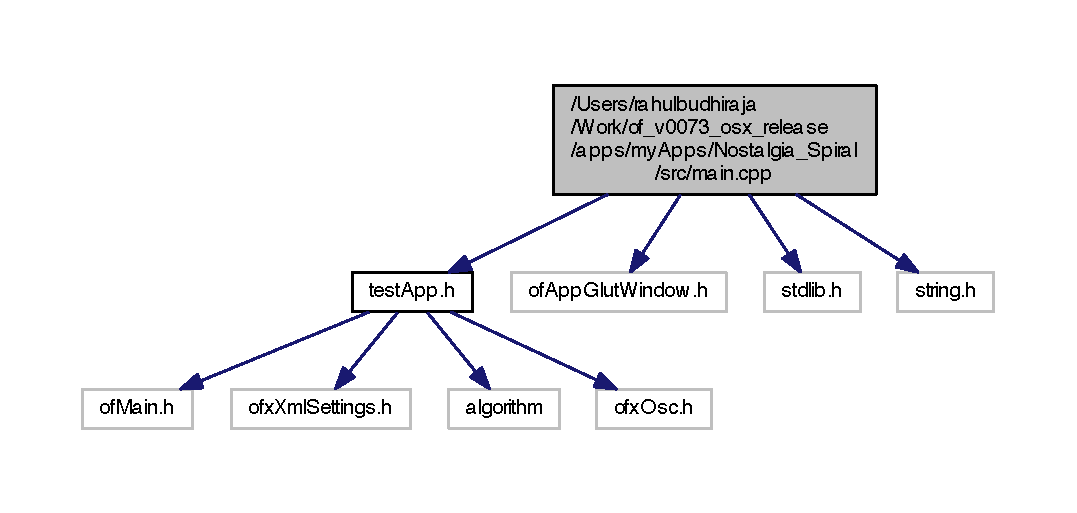
\includegraphics[width=350pt]{main_8cpp__incl}
\end{center}
\end{figure}
\subsection*{Functions}
\begin{DoxyCompactItemize}
\item 
int \hyperlink{main_8cpp_a0ddf1224851353fc92bfbff6f499fa97}{main} (int argc, char $\ast$argv\mbox{[}$\,$\mbox{]})
\end{DoxyCompactItemize}


\subsection{Function Documentation}
\hypertarget{main_8cpp_a0ddf1224851353fc92bfbff6f499fa97}{\index{main.\-cpp@{main.\-cpp}!main@{main}}
\index{main@{main}!main.cpp@{main.\-cpp}}
\subsubsection[{main}]{\setlength{\rightskip}{0pt plus 5cm}int main (
\begin{DoxyParamCaption}
\item[{int}]{argc, }
\item[{char $\ast$}]{argv\mbox{[}$\,$\mbox{]}}
\end{DoxyParamCaption}
)}}\label{main_8cpp_a0ddf1224851353fc92bfbff6f499fa97}


Definition at line 16 of file main.\-cpp.


\hypertarget{test_app_8cpp}{\section{test\-App.\-cpp File Reference}
\label{test_app_8cpp}\index{test\-App.\-cpp@{test\-App.\-cpp}}
}
{\ttfamily \#include \char`\"{}test\-App.\-h\char`\"{}}\\*
Include dependency graph for test\-App.\-cpp\-:\nopagebreak
\begin{figure}[H]
\begin{center}
\leavevmode
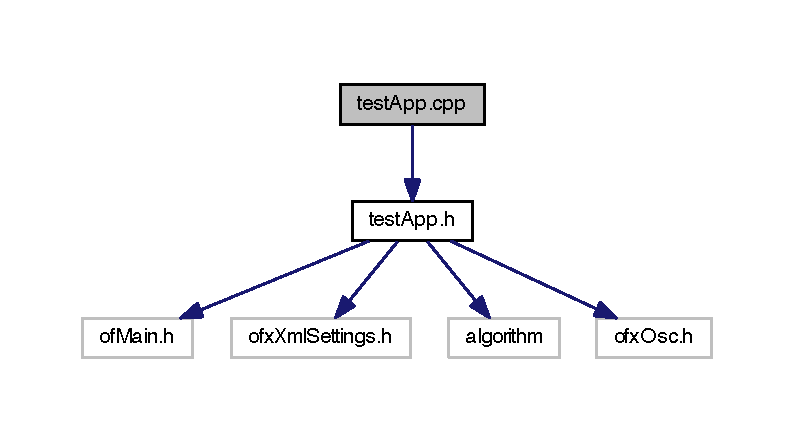
\includegraphics[width=350pt]{test_app_8cpp__incl}
\end{center}
\end{figure}

\hypertarget{test_app_8h}{\section{test\-App.\-h File Reference}
\label{test_app_8h}\index{test\-App.\-h@{test\-App.\-h}}
}
{\ttfamily \#include \char`\"{}of\-Main.\-h\char`\"{}}\\*
{\ttfamily \#include \char`\"{}ofx\-Xml\-Settings.\-h\char`\"{}}\\*
{\ttfamily \#include $<$algorithm$>$}\\*
{\ttfamily \#include \char`\"{}ofx\-Osc.\-h\char`\"{}}\\*
Include dependency graph for test\-App.\-h\-:\nopagebreak
\begin{figure}[H]
\begin{center}
\leavevmode
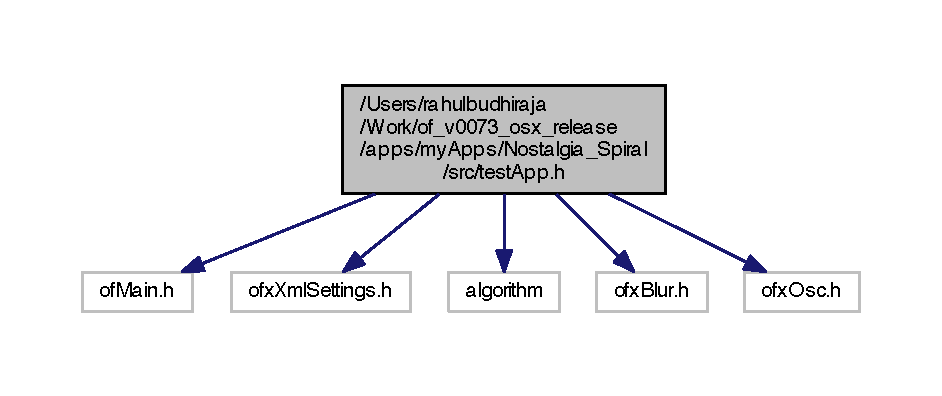
\includegraphics[width=350pt]{test_app_8h__incl}
\end{center}
\end{figure}
This graph shows which files directly or indirectly include this file\-:\nopagebreak
\begin{figure}[H]
\begin{center}
\leavevmode
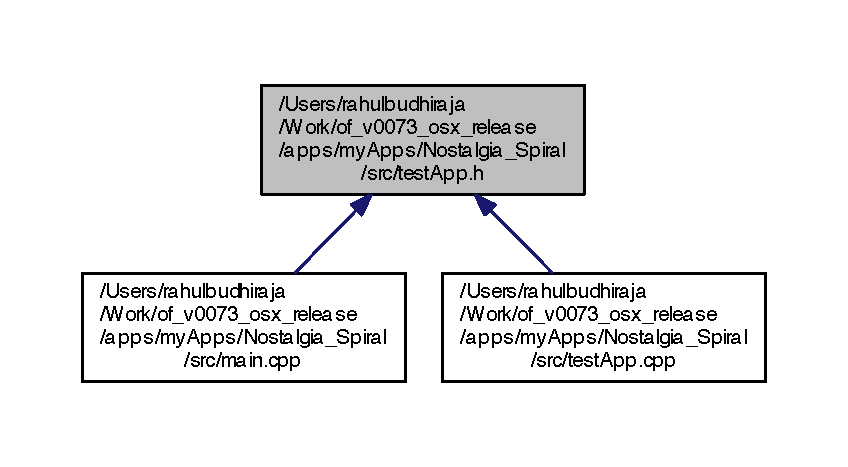
\includegraphics[width=223pt]{test_app_8h__dep__incl}
\end{center}
\end{figure}
\subsection*{Classes}
\begin{DoxyCompactItemize}
\item 
struct \hyperlink{struct_image_data}{Image\-Data}
\item 
class \hyperlink{classtest_app}{test\-App}
\end{DoxyCompactItemize}
\subsection*{Macros}
\begin{DoxyCompactItemize}
\item 
\#define \hyperlink{test_app_8h_a614217d263be1fb1a5f76e2ff7be19a2}{P\-O\-R\-T}~9000
\begin{DoxyCompactList}\small\item\em Comment U\-S\-E\-W\-I\-I to disable input from the wiimote. \end{DoxyCompactList}\item 
\#define \hyperlink{test_app_8h_a27fa4c9f9cc152f0fe3ad772b1a6b488}{Efficient\-Reorder}
\item 
\#define \hyperlink{test_app_8h_af1ac2cf7160dad9611b473a7966a8c66}{Path\-To\-Image\-Folder}~\char`\"{}/Users/rahulbudhiraja/Work/of\-\_\-v0073\-\_\-osx\-\_\-release/apps/my\-Apps/Nostalgia\-\_\-\-Spiral/bin/data/Images/\char`\"{}
\end{DoxyCompactItemize}


\subsection{Macro Definition Documentation}
\hypertarget{test_app_8h_a27fa4c9f9cc152f0fe3ad772b1a6b488}{\index{test\-App.\-h@{test\-App.\-h}!Efficient\-Reorder@{Efficient\-Reorder}}
\index{Efficient\-Reorder@{Efficient\-Reorder}!testApp.h@{test\-App.\-h}}
\subsubsection[{Efficient\-Reorder}]{\setlength{\rightskip}{0pt plus 5cm}\#define Efficient\-Reorder}}\label{test_app_8h_a27fa4c9f9cc152f0fe3ad772b1a6b488}


Definition at line 24 of file test\-App.\-h.

\hypertarget{test_app_8h_af1ac2cf7160dad9611b473a7966a8c66}{\index{test\-App.\-h@{test\-App.\-h}!Path\-To\-Image\-Folder@{Path\-To\-Image\-Folder}}
\index{Path\-To\-Image\-Folder@{Path\-To\-Image\-Folder}!testApp.h@{test\-App.\-h}}
\subsubsection[{Path\-To\-Image\-Folder}]{\setlength{\rightskip}{0pt plus 5cm}\#define Path\-To\-Image\-Folder~\char`\"{}/Users/rahulbudhiraja/Work/of\-\_\-v0073\-\_\-osx\-\_\-release/apps/my\-Apps/Nostalgia\-\_\-\-Spiral/bin/data/Images/\char`\"{}}}\label{test_app_8h_af1ac2cf7160dad9611b473a7966a8c66}


Definition at line 28 of file test\-App.\-h.

\hypertarget{test_app_8h_a614217d263be1fb1a5f76e2ff7be19a2}{\index{test\-App.\-h@{test\-App.\-h}!P\-O\-R\-T@{P\-O\-R\-T}}
\index{P\-O\-R\-T@{P\-O\-R\-T}!testApp.h@{test\-App.\-h}}
\subsubsection[{P\-O\-R\-T}]{\setlength{\rightskip}{0pt plus 5cm}\#define P\-O\-R\-T~9000}}\label{test_app_8h_a614217d263be1fb1a5f76e2ff7be19a2}


Comment U\-S\-E\-W\-I\-I to disable input from the wiimote. 

Comment A\-D\-J\-U\-S\-T\-T\-I\-M\-E\-G\-A\-P to ignore input from the wiimote and keep a standard time for which the image will be shown on the screen The ofx\-Wii\-O\-S\-C addon will listen to messages on this port 

Definition at line 19 of file test\-App.\-h.


%--- End generated contents ---

% Index
\newpage
\phantomsection
\addcontentsline{toc}{part}{Index}
\printindex

\end{document}
